\begin{samplecase}
{\bf Excitation functions: ${}^{208}$Pb (n,n'), (n,2n), (n,p) etc}\newline
Often we are not interested in only one incident energy, but in excitation 
functions of the cross sections.
If more than one incident energy is given in the file specified by the 
{\bf energy} keyword, it is helpful to have the results, for each type of cross 
section, in a table as a function of incident energy. TALYS will first 
calculate 
all quantities that remain equal for all incident energy calculations, such as 
the transmission coefficients. Next, it will calculate the results for each 
incident energy. When the calculation for 
the last incident energy has been completed, the cross sections are 
collected 
and printed as excitation functions in the output if {\bf outexcitation y} 
(which is the default if there is more than one incident energy).
Moreover, we can provide
the results in separate files: one file per reaction channel.
Consider the following input file
 
\VerbatimInput{\samples n-Pb208-xs/org/talys.inp}

which provides all partial cross sections for neutrons incident on ${}^{208}$Pb
for 46 incident energies, from 1 to 30 MeV, as given in the file 
{\em energies} that is present in this sample case directory.
In the main output file, first the results per incident energy are given.
At the end of the output file, there is an output block that begins with:  

{\small \begin{verbatim}

########## EXCITATION FUNCTIONS ###########
\end{verbatim} } \renewcommand{\baselinestretch}{1.07}\small\normalsize
\noindent
The first table contains the most important total cross sections as a function 
of incident energy. This output block begins with:

{\small \begin{verbatim}

 1. Total (binary) cross sections
 
   Energy    Non-elastic  Elastic     Total    Comp. el.  Shape el.  Reaction   
 
  1.000E+00   5.4614E-01 4.8367E+03 4.8372E+03 1.7271E+03 3.1096E+03 1.7276E+03 
  1.200E+00   6.0181E-01 4.7812E+03 4.7818E+03 1.8195E+03 2.9618E+03 1.8201E+03 
  1.400E+00   6.7627E-01 4.9406E+03 4.9413E+03 1.9485E+03 2.9921E+03 1.9492E+03 
  1.600E+00   7.6416E-01 5.2462E+03 5.2469E+03 2.1039E+03 3.1423E+03 2.1046E+03 
  1.800E+00   8.6914E-01 5.6345E+03 5.6353E+03 2.2653E+03 3.3692E+03 2.2662E+03
  2.000E+00   1.0015E+00 6.0464E+03 6.0474E+03 2.4110E+03 3.6354E+03 2.4120E+03
.....................................
\end{verbatim} } \renewcommand{\baselinestretch}{1.07}\small\normalsize
\noindent
Next, the binary cross sections are printed.
This output block begins with:

{\small \begin{verbatim}

 2. Binary non-elastic cross sections (non-exclusive)
 
   Energy     gamma      neutron    proton     deuteron   triton     helium-3   
 
  1.000E+00   1.9672E-01 0.0000E+00 0.0000E+00 0.0000E+00 0.0000E+00 0.0000E+00 
  1.200E+00   2.4416E-01 0.0000E+00 0.0000E+00 0.0000E+00 0.0000E+00 0.0000E+00 
  1.400E+00   3.0773E-01 0.0000E+00 0.0000E+00 0.0000E+00 0.0000E+00 0.0000E+00 
  1.600E+00   3.8879E-01 0.0000E+00 0.0000E+00 0.0000E+00 0.0000E+00 0.0000E+00 
  1.800E+00   4.9418E-01 0.0000E+00 0.0000E+00 0.0000E+00 0.0000E+00 0.0000E+00 
  2.000E+00   6.3274E-01 0.0000E+00 0.0000E+00 0.0000E+00 0.0000E+00 0.0000E+00 
.....................................
\end{verbatim} } \renewcommand{\baselinestretch}{1.07}\small\normalsize
\noindent
Next, the total particle production cross sections are printed.
Parts of this output block look as follows:

{\small \begin{verbatim}

 3. Total particle production cross sections
 
 gamma    production     

 Energy   Cross section Multiplicity
  
  1.000E+00 2.47648E-01 1.43346E-04
  1.200E+00 3.14552E-01 1.72825E-04
  1.400E+00 4.06594E-01 2.08595E-04
  1.600E+00 5.23101E-01 2.48546E-04   
  1.800E+00 6.76670E-01 2.98596E-04
  2.000E+00 8.80247E-01 3.64945E-04
  2.200E+00 1.14449E+00 4.52788E-04
  2.400E+00 1.48925E+00 5.70753E-04      
.....................................
 neutron  production

 Energy   Cross section Multiplicity

  1.000E+00 4.26190E-03 2.46692E-06
  1.200E+00 9.15765E-03 5.03151E-06
  1.400E+00 1.71089E-02 8.77738E-06
  1.600E+00 3.18516E-02 1.51339E-05
  1.800E+00 5.42068E-02 2.39200E-05
  2.000E+00 8.89349E-02 3.68719E-05
  2.200E+00 1.41778E-01 5.60908E-05
  2.400E+00 2.20738E-01 8.45971E-05
  2.600E+00 3.30648E-01 1.24267E-04
  2.800E+00 3.16809E+02 1.17802E-01
.....................................
\end{verbatim} } \renewcommand{\baselinestretch}{1.07}\small\normalsize
\noindent
Next in the output are the residual production cross sections. The output
block begins with:

{\small \begin{verbatim}

 4. Residual production cross sections
  
 Production of Z= 82 A=209 (209Pb) - Total
  
 Q-value    =   3.937307
 E-threshold=   0.000000
  
 Energy   Cross section 
  
  1.000E+00 1.92452E-01            
  1.200E+00 2.35002E-01            
  1.400E+00 2.90625E-01            
  1.600E+00 3.56940E-01            
  1.800E+00 4.39971E-01            
  2.000E+00 5.43801E-01            
  2.200E+00 6.70818E-01            
  2.400E+00 8.26660E-01            
  2.600E+00 1.02344E+00 
.....................................
\end{verbatim} } \renewcommand{\baselinestretch}{1.07}\small\normalsize
\noindent
and the remaining isotopes follow in decreasing order of mass and isotope.

The final part of the output, for this input file at least, concerns the
exclusive reaction cross sections. This output block begins with:

{\small \begin{verbatim}

 6. Exclusive cross sections

     Emitted particles     reaction
   n   p   d   t   h   a
   0   0   0   0   0   0       (n,g)            

 Q-value    =   3.937307
 E-threshold=   0.000000
  
 Energy   Cross section Gamma c.s. c.s./res.prod.cs
  
  1.000E+00 1.92452E-01 3.48872E-01 1.00000E+00
  1.200E+00 2.35002E-01 4.35691E-01 1.00000E+00
  1.400E+00 2.90625E-01 5.54769E-01 1.00000E+00
  1.600E+00 3.56940E-01 6.97846E-01 1.00000E+00
  1.800E+00 4.39971E-01 8.82793E-01 1.00000E+00
  2.000E+00 5.43801E-01 1.12074E+00 1.00000E+00
.....................................
     Emitted particles     reaction
   n   p   d   t   h   a
   1   1   0   0   0   0       (n,np)           

 Q-value    =  -8.003758   
 E-threshold=   8.042576


 Energy   Cross section Gamma c.s. c.s./res.prod.cs

  1.000E+00 0.00000E+00 0.00000E+00 0.00000E+00                                 
  1.200E+00 0.00000E+00 0.00000E+00 0.00000E+00                                 
  1.400E+00 0.00000E+00 0.00000E+00 0.00000E+00                                 
  1.600E+00 0.00000E+00 0.00000E+00 0.00000E+00                                 
  1.800E+00 0.00000E+00 0.00000E+00 0.00000E+00                                 
  2.000E+00 0.00000E+00 0.00000E+00 0.00000E+00                                 
  2.200E+00 0.00000E+00 0.00000E+00 0.00000E+00                   
.....................................
  2.000E+01 3.12374E+00 2.18877E+00 5.08526E-01
  2.200E+01 8.55243E+00 8.69348E+00 6.06418E-01
  2.400E+01 1.70454E+01 2.30865E+01 6.79074E-01
  2.600E+01 2.70534E+01 4.51648E+01 7.31295E-01
  2.800E+01 3.62134E+01 6.92506E+01 7.66934E-01
  3.000E+01 4.31314E+01 9.02171E+01 7.89711E-01
\end{verbatim} } \renewcommand{\baselinestretch}{1.07}\small\normalsize
\noindent
For plotting data, or processing into ENDF-6 data files, it is more practical
to have the data in individual output files. Note that, since 
{\bf filechannels y}, several files with names as e.g. {\em xs200000.tot} have 
been created in your working directory. These files contain the entire
excitation function per reaction channel.
Besides these 
exclusive cross sections, residual production cross section files are produced
({\bf fileresidual y}).
Note that for this reaction, {\em rp082207.tot} and {\em xs200000.tot} 
obviously have equal contents. 

We illustrate this sample case with various comparisons with measurements. Since
{\bf filetotal y}, a file {\em total.tot} is created with, among others, the 
total cross section. The resulting curves are shown in Figs.~\ref{pbpart1} and 
\ref{pbpart2}.
\end{samplecase}
\begin{figure}
\vspace*{-5mm}
\centerline{
\centering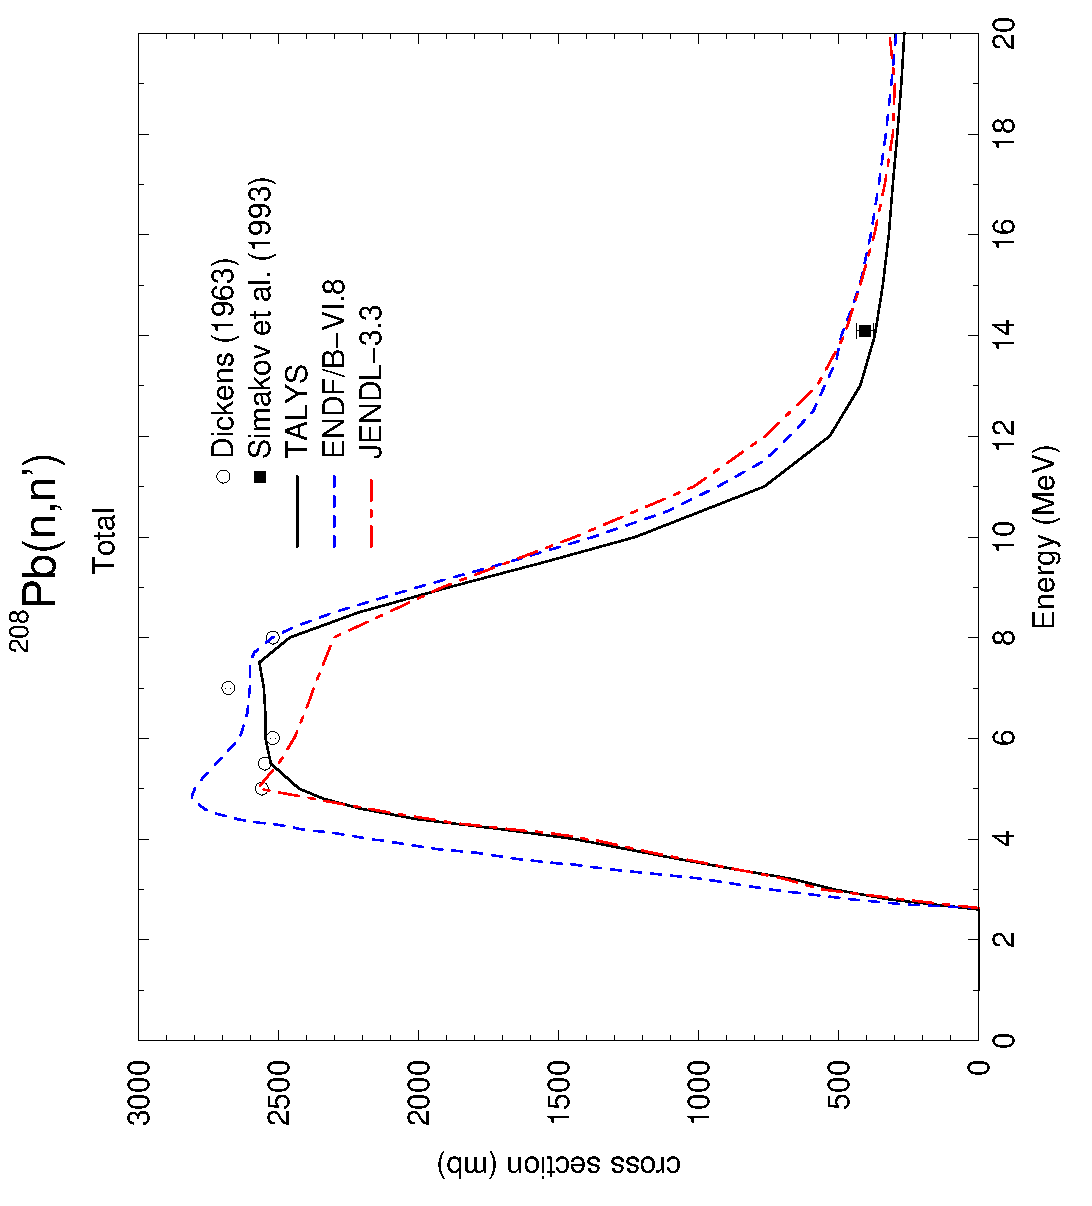
\includegraphics[scale=0.5,angle=270]{MT4} \centering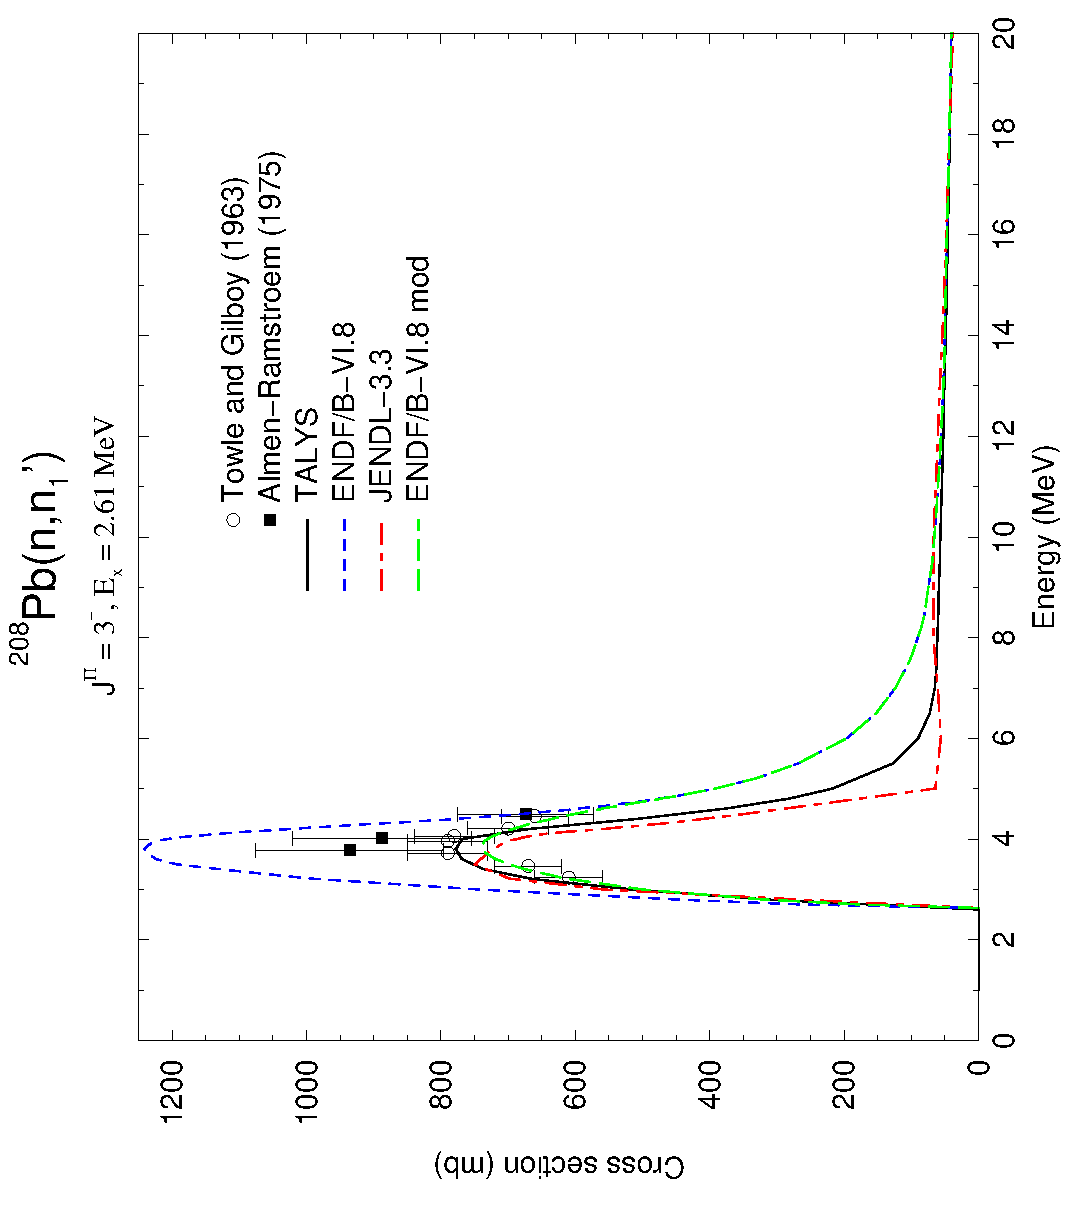
\includegraphics[scale=0.5,angle=270]{MT51}
}
\centerline{
\centering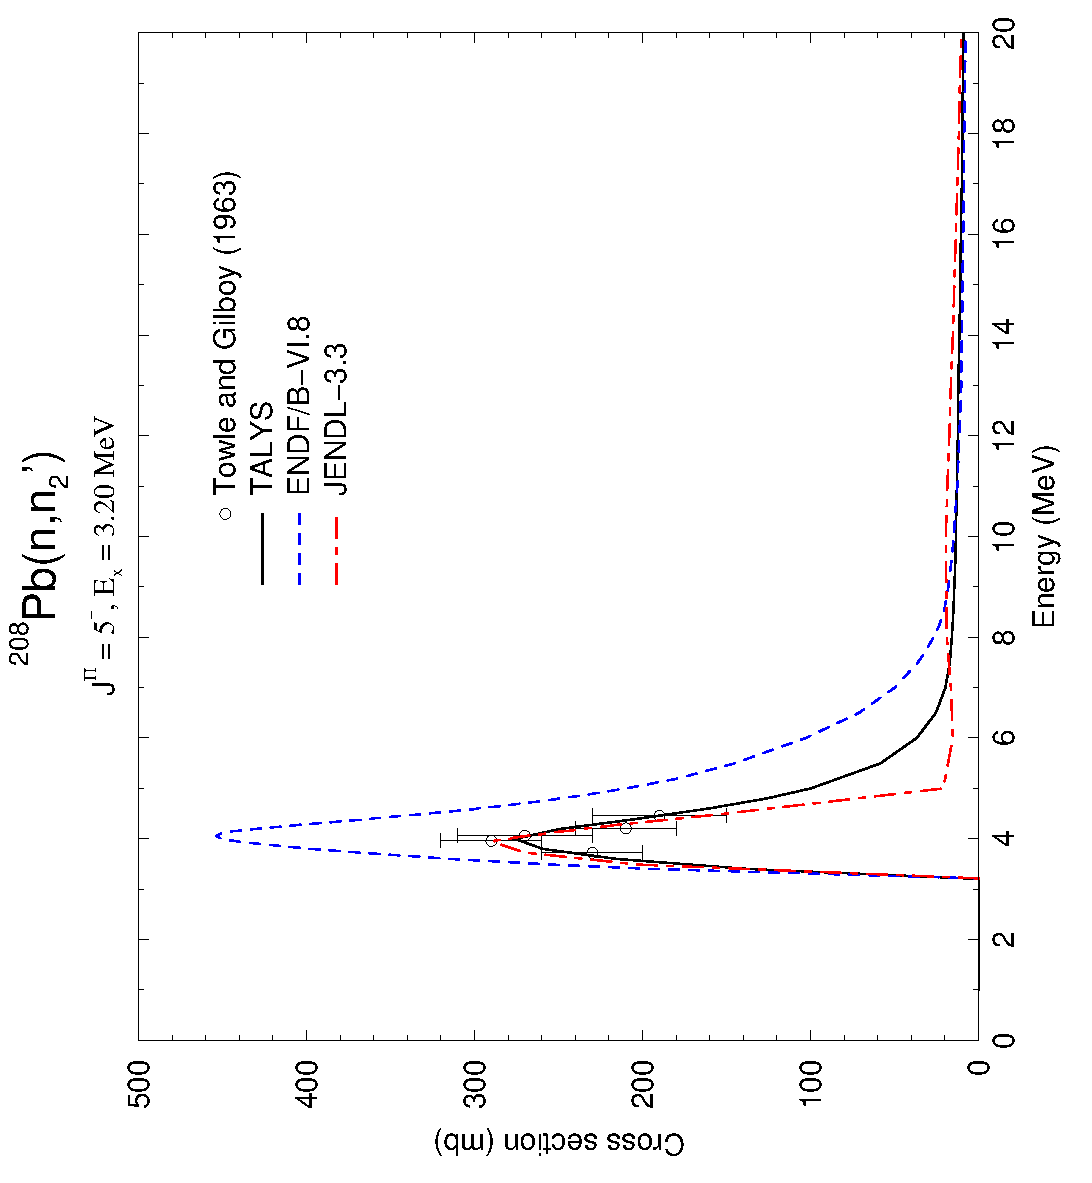
\includegraphics[scale=0.5,angle=270]{MT52} \centering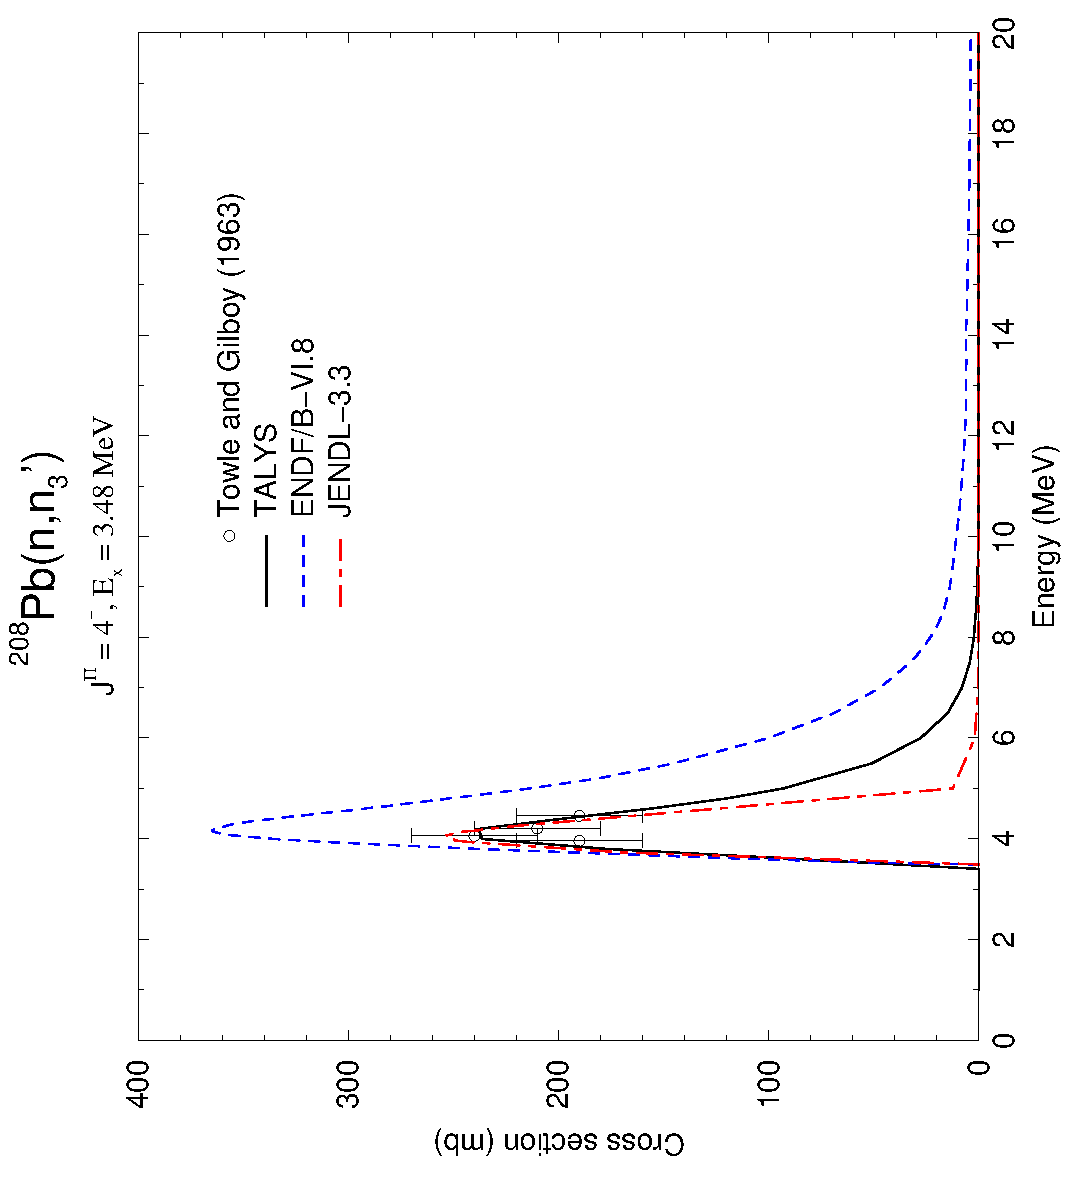
\includegraphics[scale=0.5,angle=270]{MT53}
}
\caption{Partial cross sections for neutrons incident on ${}^{208}$Pb.}
\label{pbpart1}
\end{figure}
\begin{figure}
\vspace*{-15mm}
\centerline{
\centering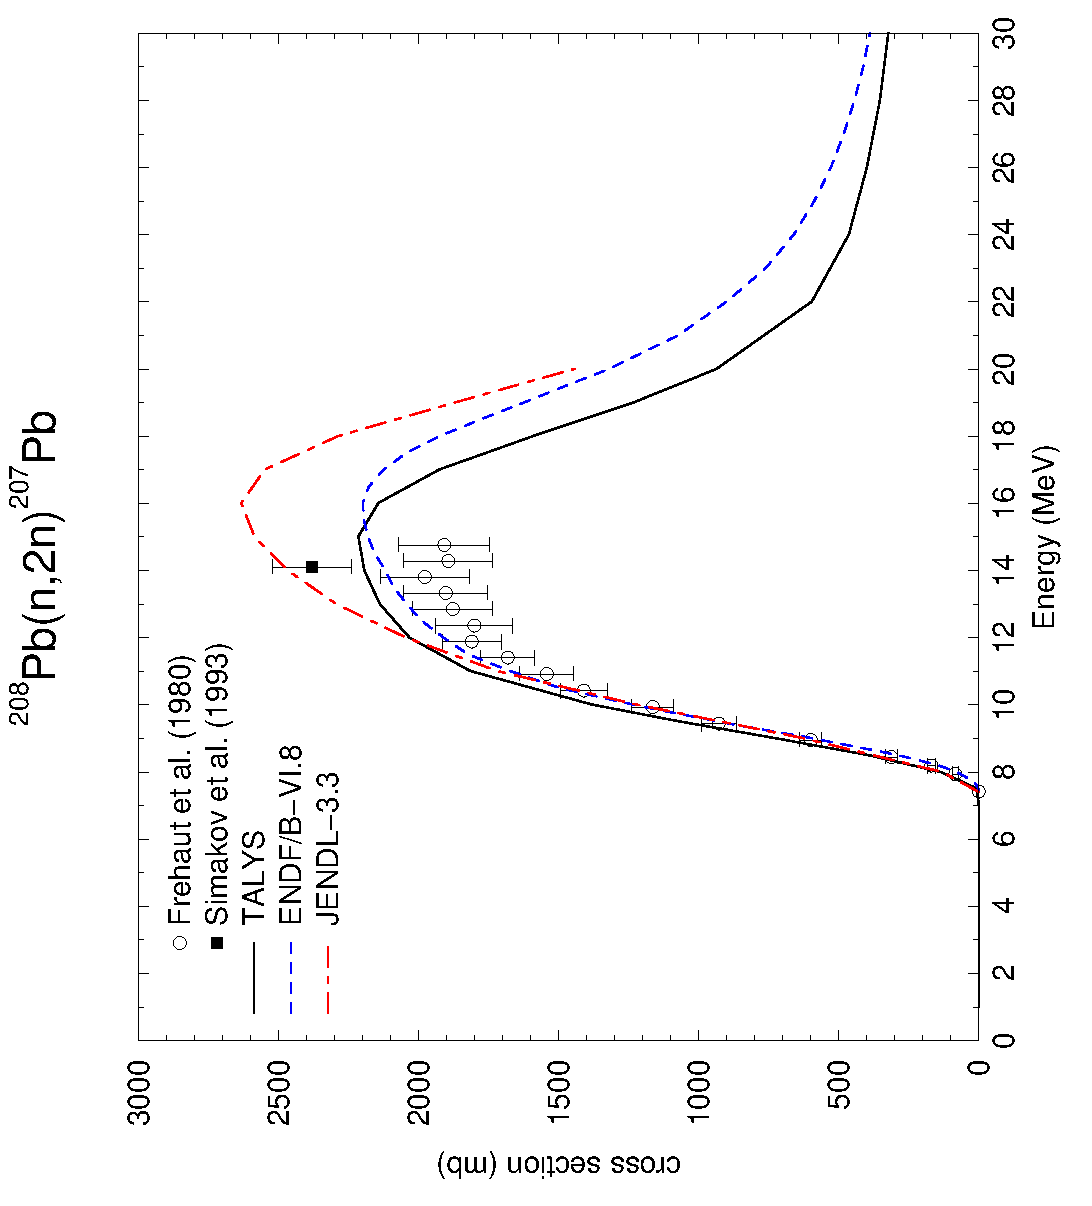
\includegraphics[scale=0.5,angle=270]{MT16} \centering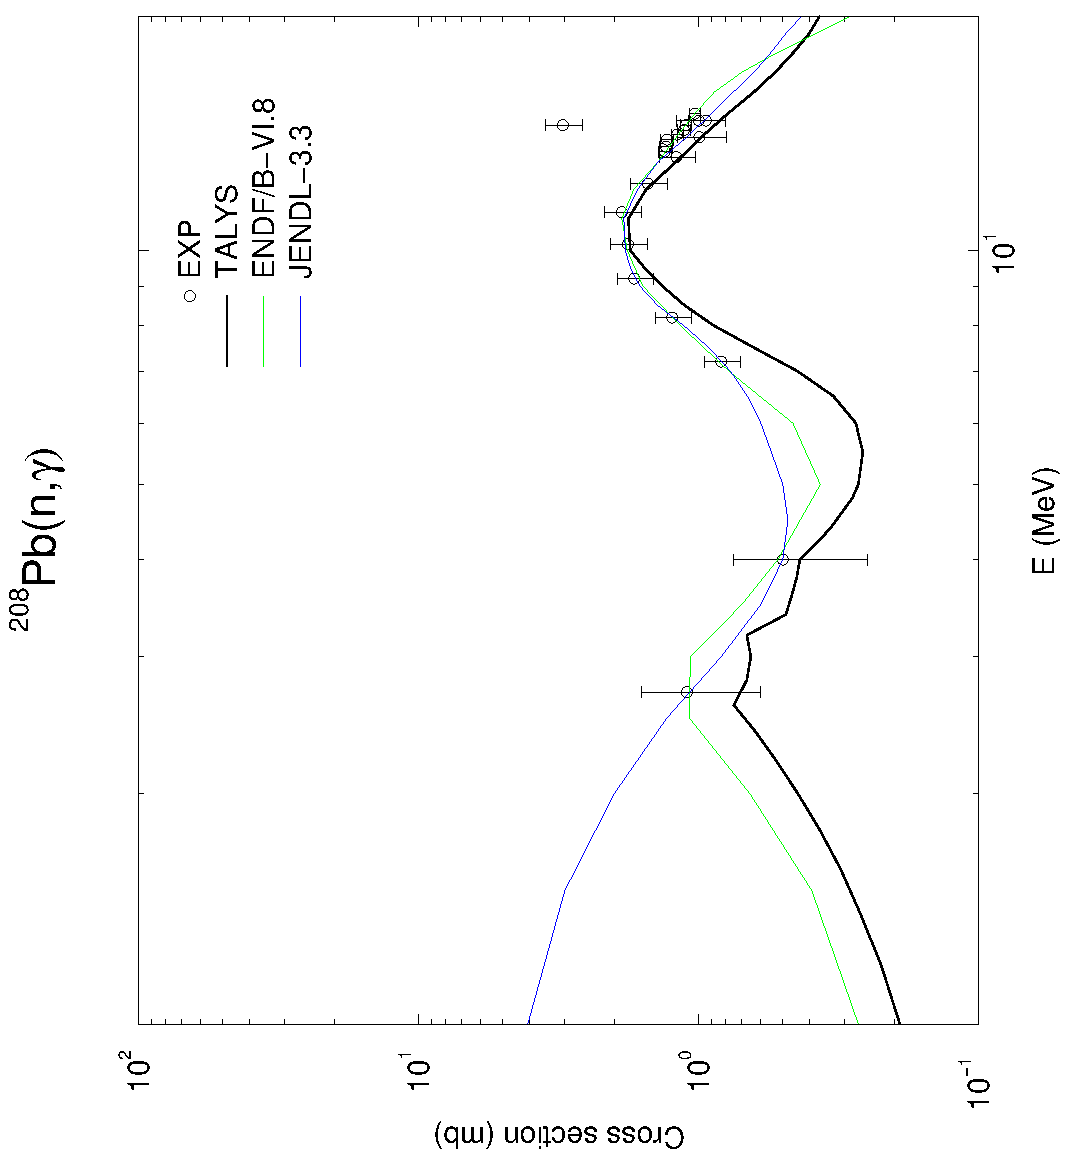
\includegraphics[scale=0.5,angle=270]{MT102}
}
\centerline{
\centering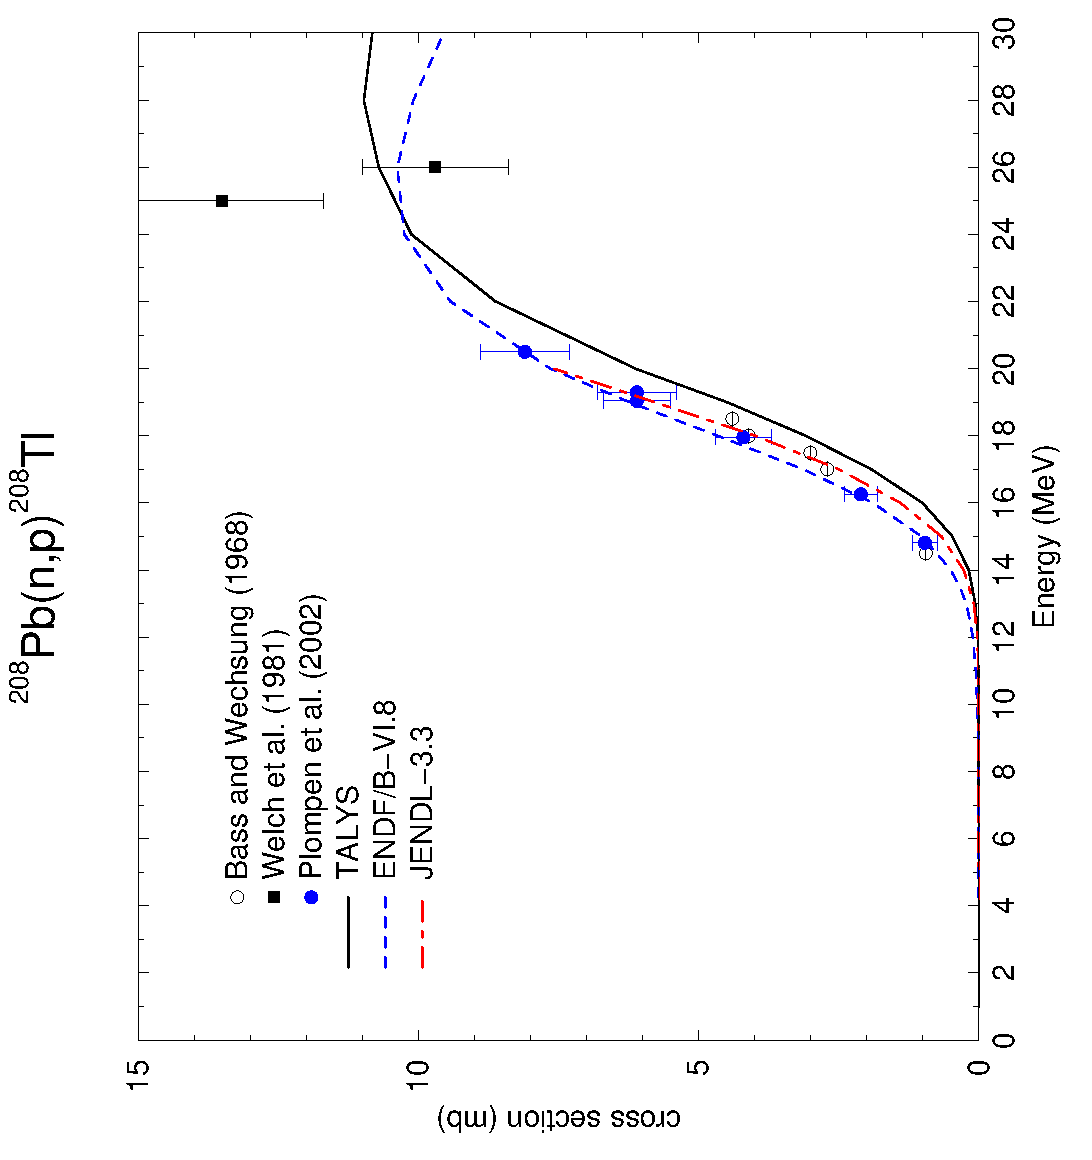
\includegraphics[scale=0.5,angle=270]{MT103} \centering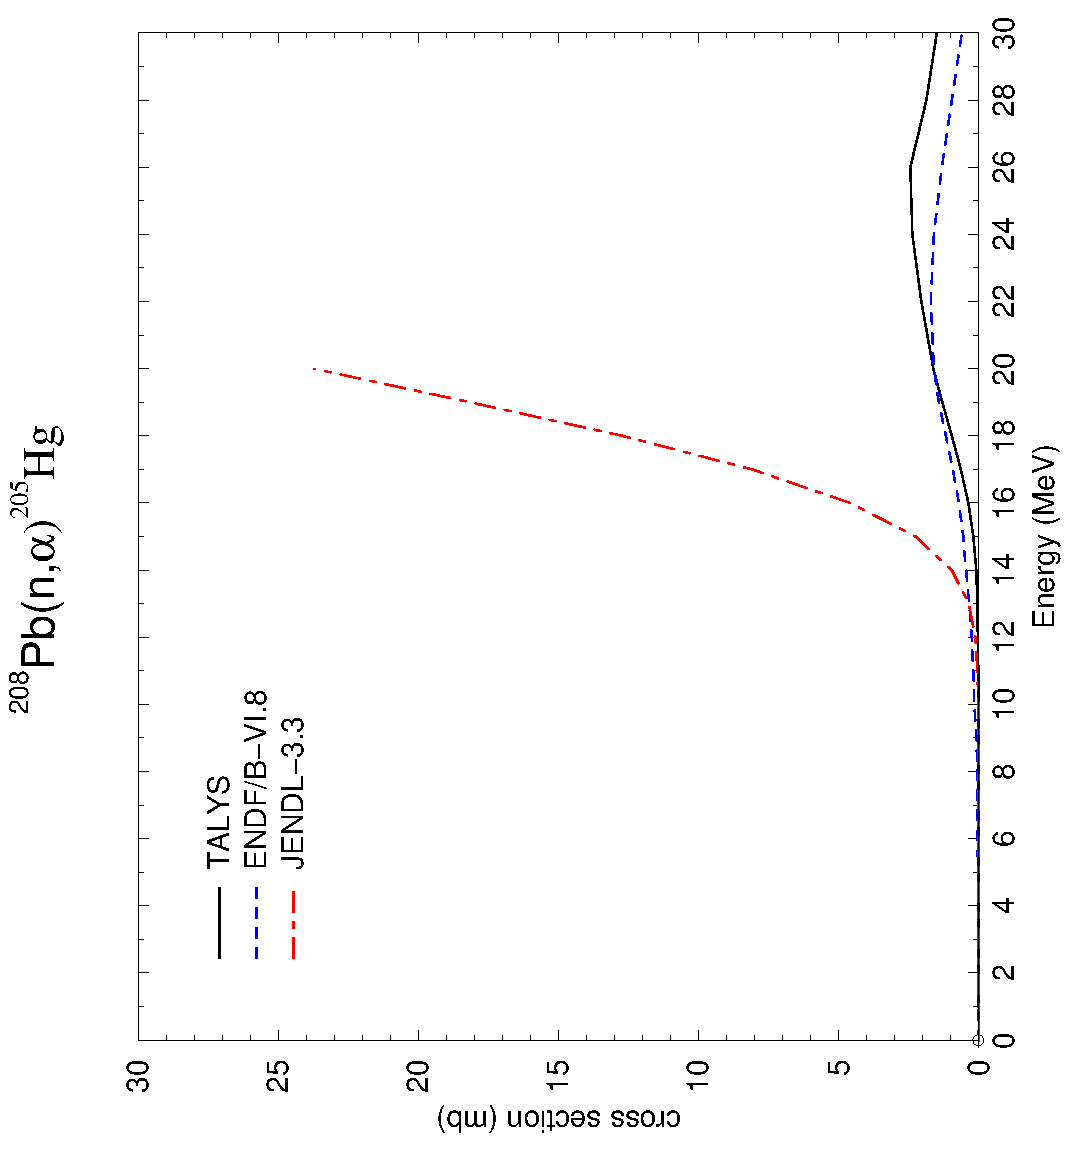
\includegraphics[scale=0.5,angle=270]{MT107}
}
\caption{Partial cross sections for neutrons incident on ${}^{208}$Pb.}
\label{pbpart2}
\end{figure}
